%chktex-file 1 
%chktex-file 8

\documentclass[12pt,a4paper,hidelinks]{article}
\usepackage[british]{babel}

%%MUST STAY HERE
\usepackage[svgnames, table]{xcolor}
%%
\usepackage{algorithm}
\usepackage{algpseudocode}
\usepackage{amsfonts}
\usepackage{amsthm}
\usepackage{amsmath}
\usepackage{array}
\usepackage{amssymb}
\usepackage{arydshln}

\usepackage{bbding}
\usepackage{booktabs}

\usepackage[labelfont={bf,sf,footnotesize,color=pblue},textfont={footnotesize}, margin={40pt,40pt}]{caption}

\usepackage{eurosym}

\usepackage[T1]{fontenc}
\usepackage{fullpage}
\usepackage{graphicx}

\usepackage[colorlinks = true,
            linkcolor = pdarkerblue,
            urlcolor  = gblue,
            citecolor = gblue,
            anchorcolor = blue]{hyperref}%%Must stay here
\usepackage{caption}
\usepackage{cleveref}
%%
\usepackage{hhline}
\usepackage{listings}
\usepackage{lipsum}

\usepackage{mathrsfs}
\usepackage{mathtools}
\usepackage{mdframed}
\usepackage{minted}
\usepackage{multicol}
\usepackage{multirow}

\usepackage[numbers,sort]{natbib}
\usepackage{navigator}

\usepackage{palatino}
\usepackage{pifont}
\usepackage{pgffor}
\usepackage{pgfplots}
\usepackage{pgfplotstable}
\usepackage{placeins}

\usepackage{sectsty}
\usepackage{siunitx}
\usepackage{subfig}

\usepackage{tabularx}
\usepackage[many]{tcolorbox}
\usepackage{tikz}
\usepackage{todonotes}

\usepackage{verbatim}

\usepackage{wrapfig}

\usepackage{xinttools}
\usepackage{xcolor}

%%%~~~~~~~~~~~~~~~~~~~~~~~~Fonts~~~~~~~~~~~~~~~~~~~~~~~%%%


%%%~~~~~~~~~~~~~~~~~~~~~~~~Colours~~~~~~~~~~~~~~~~~~~~~%%%
\definecolor{gblue}{HTML}{000099}
\definecolor{pblue}{HTML}{00004d}%{0000FF}
\definecolor{pdarkblue}{HTML}{000080}
\definecolor{pdarkerblue}{HTML}{000066}
%\definecolor{veryblue}{HTML}{00004d}

%~~~~~~~~~~~~~~~~~~~~~~~~~~~~~Tikz~~~~~~~~~~~~~~~~~~~~~~~~~~~~~%
\usetikzlibrary{calc}
\usetikzlibrary{shapes,arrows,arrows.meta}
\usetikzlibrary{automata,positioning}
\usetikzlibrary{spy,backgrounds}
\usetikzlibrary{matrix,positioning,arrows.meta,arrows}
\usetikzlibrary{fadings}
\usetikzlibrary{positioning}
\usetikzlibrary{fit}

\newcommand{\nomefico}{\textbf{nomeFicoDaScegliere}}
\newcommand{\github}{\texttt{https://github.com/magemma/question-answering}}
\newcommand{\app}{\texttt{https://link-alla-app}}

\pgfplotsset{compat=1.15}

\sectionfont{\bf \Large \color{pblue}}
\subsectionfont{\bf \color{pdarkblue}}
\subsubsectionfont{\bf \color{pdarkerblue}}

\newtcolorbox{myframe}[3][]{
  width=\linewidth-20pt,
  boxrule=0.5pt,
  fonttitle=\bfseries,
  colback=#3!20!white,
  colframe=#3!80,
  title={#2},
  center,
  enlarge top by=2\parsep,%     equivalent to mdframed 'skipabove'
  enlarge bottom by=2\parsep,%
  #1
}%

\newtcolorbox{mydisclaimer}[2][]{
  width=\linewidth-1pt,
  boxrule=0.3pt,
  fonttitle=\bfseries,
  colback=pdarkblue!20,
  colframe=pdarkblue,
  title={#2},
  #1
}%


%%%%%%%%%%%%%%%%%%%%%%%%%%%%%%%%%%%%%%%%%%%%%%%%%%%%%%%%%%%%%%%%%%%%%%%%%%%%%%%%%%

\begin{document}

\begin{mydisclaimer}{{\large \ding{74}} \,  Osservazioni}
\begin{itemize}
    \item Gli errori qui sopra e di compilazione sono dovuti a questo rettangolo blu, che tanto sparisce
    \item L'abstract adesso conta 267 parole. Di solito gli abstract non sono piu' lunghi di 300
    \item Il nome del nostro strumento di QA sta in una macro, per usarlo nel report scrivere \texttt{\textbackslash nomefico}
    \item Il link al repo github sta in una macro, per usarlo scrivere \texttt{\textbackslash github}
    \item Il link alla pagina web per QA (ancora da definire) sta in una macro, chiamata \texttt{\textbackslash app}
\end{itemize}
\end{mydisclaimer}

\newpage

\begin{titlepage}
    \centering
    \begin{minipage}{0.22\textwidth}%
        
\includegraphics[width=\linewidth]{pics/Cherubino.jpg}
    \end{minipage}\hspace{10pt}
    \begin{minipage}{0.6\textwidth}%
        \flushright
        \large
        \vspace{0.8cm}
        \textsc{\color{pblue}%
        \nomefico\\
        a Bert-based, open domain\\
        question answering system}
        
\begin{tikzpicture}%
            \draw[thick, brown] (0.1,0)--(0.99\textwidth,0);%   
        \end{tikzpicture}%
    \end{minipage}%

    
    %{\color{pblue} \textsc{ \Large Human Language Techonlogies}}
    
    %\vspace{0.5cm}
    
    %{\color{pblue} \textsc{ A.Y. 2018-2019}}
    
    \vspace{0.3cm}
    
    Gabriele Barreca, Mario Bonsembiante {\small and} Gemma Martini
    
    %\vspace{0.4cm}
    
    {\scriptsize University of Pisa}
    
    \vspace{0.5cm}
    
    \abstract{
    \scriptsize
    Question answering (QA) systems can be seen as information retrieval systems which aim is to respond to queries, stated in natural language, by returning short answers or long sentences.
    The ``so-called'' \emph{open domain QA task} adds the challenge of understanding if the answer to the selected question may or may not be found in a given paragraph, which content has been buried within large text corpora, such as Wikipedia.

    \vspace{0.1cm}

    Building such systems for practical applications has historically been quite challenging and involved.
    The spectrum of possible answers given a question and a paragraph, moves from the ``simple'' \emph{yes/no answers} to the longer and more articulated \emph{long answers}, to then get to a trade-off between expressive power and succinctness, the ``so-called'' \emph{short answers}, which aim to enclose the answer in a single and possibly short sentence.
    
    \vspace{0.1cm}
    
    In this paper, we present a BERT-based implementation that solves an open domain QA task, providing all the three categories of answers listed above, with particular attention on the most widely studied kind, i.e. short answers.
    We achieve pretty good results, although not as good as the state-of-the-art, that was not the purpose of this work.
    
    As expected and already stated in previous work, we conclude that predicting long answers per se is pretty unreliable, while much better results are achieved if the short answer is predicted and then enlarged with the whole paragraph it lies in, from the original text.
}
    
    \vspace{1cm}
    
    
\begin{tikzpicture}%
        \draw[thick, brown] (0,0)--(0.8\textwidth,0);%   
    \end{tikzpicture}%
    
    \vspace{-0.5cm}
    \tableofcontents

    \vspace{0.36cm}

    
\begin{tikzpicture}%    
        \draw[thick, brown] (0,0)--(0.8\textwidth,0);%   
    \end{tikzpicture}%

    %{\large \today}
    \vfill
\end{titlepage}

%%%%%%%%%%%%%%%%%%%%%%%%%%%%%%%%%%%%%%%%%%%%%%%%%%%%%%%%%%%%%%%%%%

%\thispagestyle{empty}
\newpage
\setcounter{page}{1}

%%%%%%%%%%%%%%%%%%%%%%%%%%%%%%%%%%%%%%%%%%%%%%%%%%%%%%%%%%%%%%%%%%
\section{Introduction}\label{sec:intro}
%%%%%%%%%%%%%%%%%%%%%%%%%%%%%%%%%%%%%%%%%%%%%%%%%%%%%%%%%%%%%%%%%%

Moreover, we uploaded a Python implementation on \href{cia}{this} \footnote{ciap} GitHub repository and we integrated it with a straightforward UI, available at \href{www.gemmamartini.it}{www.gemmamartini.it}.

\todo[inline]{aggiungere una frase in cui si dice che cosa si trova in quali sezioni}


%%%%%%%%%%%%%%%%%%%%%%%%%%%%%%%%%%%%%%%%%%%%%%%%%%%%%%%%%%%%%%%%%%
\section{The architecture}\label{sec:model}
%%%%%%%%%%%%%%%%%%%%%%%%%%%%%%%%%%%%%%%%%%%%%%%%%%%%%%%%%%%%%%%%%%
Before digging into the details of the machine learning core of our BERT-based QA system, let us define the outline of the responsive QA tool we developed.

In \Cref{fig:application_dataflow} there is a pictorial representation of how the user interacts with the system, how it processes the information (server side) and how it prompts the results.

\begin{figure}[ht!]
    \centering
    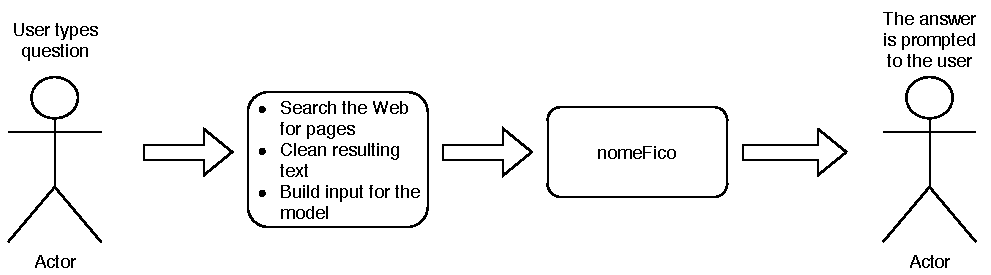
\includegraphics[width=0.9\textwidth]{report/pics/tool_dataflow.pdf}
    \caption{The full functioning of \nomefico, combined with an effective user interface.}
    \label{fig:application_dataflow}
\end{figure}

\todo[inline]{Aggiungere descrizione con immagini del workflow dell'applicazione, con un esempio che funziona, magari creando una sottosezione.}

\subsection{\nomefico}\label{subsec:nomefico}
We are now ready to discuss the implementation of \nomefico.

We decided to tackle the open domain QA task problem creating a stack of two neural networks, forming a two-layer architecture, see \Cref{fig:broad_architecture}.
The first layer is built using BERT's \cite{devlin2018bert} checkpoints, while the second layer is a neural networks that uses BERT's embeddings and the Natural Questions (NQ) \cite{kwiatowski} dataset \footnote{Some qualities of NQ are the following: (1) the questions were formulated by people out of genuine curiosity or out of need for an answer to complete another task, (2) the questions were formulated by people before they had seen the document that might contain the answer, (3) the documents in which the answer is to be found are much longer than the documents used in some of the existing question answering challenges.} with the aim of obtaining the start position and end position of the answer in the given paragraph.

\begin{figure}[ht!]
    \centering
    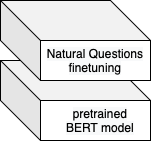
\includegraphics[scale=.9]{pics/broad_architecture.png}
    \caption{.}
    \label{fig:broad_architecture}
\end{figure}



Let us dig into details a bit more and explain how the BERT layer works.



At this point, we assume that the system receives as input two textual items, the first one is the question and the second one is the paragraph that is supposed to contain the answer

\todo[inline]{short?long?}

In this section the tools used in the project are described.

%%%%%%%%%%%%%%%%%%%%%%%%%%%%%%%%%%%%%%%%%%%%%%%%%%%%%%%%%%%%%%%%%%
\section{Experimental results}\label{sec:experimental_results}
%%%%%%%%%%%%%%%%%%%%%%%%%%%%%%%%%%%%%%%%%%%%%%%%%%%%%%%%%%%%%%%%%%


%%%%%%%%%~~~~~~~~~~~~~~~~~~~~~~~~~~%%%%%%%%%%
\subsection{Hardware}
%%%%%%%%%~~~~~~~~~~~~~~~~~~~~~~~~~~%%%%%%%%%%


%%%%%%%%%~~~~~~~~~~~~~~~~~~~~~~~~~~%%%%%%%%%%
\subsection{Hyper-parameters values}
%%%%%%%%%~~~~~~~~~~~~~~~~~~~~~~~~~~%%%%%%%%%%

%%%%%%%%%%%%%%%%%%%%%%%%%%%%%%%%%%%%%%%%%%%%%%%%%%%%%%%%%%%%%%%%
\section{Future work}\label{sec:future_work}
%%%%%%%%%%%%%%%%%%%%%%%%%%%%%%%%%%%%%%%%%%%%%%%%%%%%%%%%%%%%%%%%
Use a binary classification layer to check if the answer is ``plausible'' (i.e. the meanings in the question are covered in the answer), as done by \cite{Hu2019ReadV} and \cite{Back2020NeurQuRI}.



%%%%%%%%%%%%%%%%%%%%%%%%%%%%%%%%%%%%%%%%%%%%%%%%%%%%%%%%%%%%%%%%
\section{Conclusions}\label{sec:conclusions}
%%%%%%%%%%%%%%%%%%%%%%%%%%%%%%%%%%%%%%%%%%%%%%%%%%%%%%%%%%%%%%%%

%%%%%%%%%%%%%%%%%%%~~~~~~~~~~~~~~~~~~~~~~~~~~%%%%%%%%%%%%%%%%%%%%
\subsection{All references}

\begin{itemize}
  \item kbqa~\cite{kbqa}    
  \item coqa~\cite{coqa}
  \item collobert~\cite{Collobert}
  \item vaswani~\cite{vaswani}
  \item weston1~\cite{weston-tracking}
  \item weston2~\cite{weston-reading}
  \item alberti 2019~\cite{alberti}
  \item kwiatowski 2019~\cite{kwiatowski}
  \item chen~\cite{chen}
  \item liu purple~\cite{liu-purple}
  \item liu yellow~\cite{liu-yellow}
  \item RoBERTa~\cite{roberta}
\end{itemize}


\bibliographystyle{unsrt}
\bibliography{references}

\end{document} 
